\documentclass[xcolor=dvipsnames, xcolor=table]{beamer} % Classe de documento para apresentações
\usepackage{listings}
\usepackage{listings}\usetheme{Berlin}
\usecolortheme{beaver}
\usepackage{textpos}
\usepackage{color}
\usepackage{wasysym}
\renewcommand\tabcolsep{4pt}
\usepackage{csquotes} 
\usepackage{wrapfig}
\usepackage{microtype}
\usepackage[labelfont=bf]{caption}
\usepackage{epigraph}
\usepackage[english]{babel}
\usepackage{float}
\usepackage{hyperref}
\usepackage{amsmath}
\newcommand{\dd}[1]{\mathrm{d}#1}
\usepackage{amsfonts}
\usepackage{amssymb}
\usepackage{amsbsy}
\usepackage{graphicx}
\usepackage{mathtools}

\usepackage{booktabs}

\usepackage{adjustbox}
\hypersetup{pdfpagemode=FullScreen} % para o pdf abrir automaticamente em modo full screen
\setbeamertemplate{caption}[numbered] % para numerar as tabelas
\usepackage{subcaption}
\usepackage[none]{hyphenat} 
\usepackage{bm} %%% bold vectors
\usepackage{tabularx}  
\usepackage{tikz}




\setbeamercolor{author in head/foot}{fg=Maroon}     % cor do nome do autor no rodape
\setbeamercolor{institute in head/foot}{fg=Maroon}  % cor do nome do ISEG no rodape
\setbeamercolor{frametitle}{fg=Maroon, bg=black!9} % cor da letra e do fundo fa faixa com o nome de cada slide
\setbeamercolor{caption name}{fg=Maroon, bg=black!9}
\setbeamercolor*{title}{fg=white, bg=Maroon}          % cor do titulo e da caixa de titulo na capa
\setbeamercolor{itemize item}{fg=Maroon}               % cor dos bullets do ambiente \itemize 


\makeatletter % criaçao de um ambiente sem TOC no cabeçalho do slide
\newenvironment{noheadline}{
\setbeamertemplate{headline}{}
\addtobeamertemplate{frametitle}{\vspace*{-0.9\baselineskip}}{}
}{}
\makeatother

\usepackage[beamer,customcolors]{hf-tikz}

\tikzset{hl/.style={
    set fill color=red!80!black!40,
    set border color=red!80!black,
  },
}


\title[Non-Numeric Values]{Non-Numeric Values}
\author[Pedro Fonseca]{\textbf {Pedro Fonseca}}
\titlegraphic{
\includegraphics[width=1.5cm]{yes}}
\institute[Introduction to R]{\textbf {Introduction to R}}
\date{\today}


% position the yes
\addtobeamertemplate{frametitle}{}{%
\begin{textblock*}{100mm}(.85\textwidth,-.9cm)

\includegraphics[scale=.05]{yes}
\end{textblock*}}



%%%%%%%%%%%%% Ambiente de teorema/definição com as cores do ISEG %%%%%%

\makeatletter
\def\th@mystyle{%
    \normalfont % body font
    \setbeamercolor{block title example}{bg=Maroon,fg=white}
    \setbeamercolor{block body example}{bg=black!9,fg=black}
    \def\inserttheoremblockenv{exampleblock}
  }
\makeatother
\theoremstyle{mystyle}
\newtheorem*{defi}{Definição}

\setbeamertemplate{defis}[numbered]



%%%%%%%%%%%%%%%% Bibliografia %%%%%%%%%%%%%%%%%%%%%%%

\usepackage{url}
\usepackage[style=authoryear, bibencoding=utf8, minnames=1, maxnames=3,
maxbibnames=99,backref=true, natbib=true, dashed=false, terseinits=true, 
firstinits=true, uniquename=false, uniquelist=true, labeldate=true, 
doi=false, isbn=false, natbib=true, backend=biber]{biblatex}
\DefineBibliographyStrings{english}{%
    backrefpage = {Cited on page},
    backrefpages = {Cited on pages},
}
% Change the default formatting to be more "statistical"
\DeclareFieldFormat{url}{\url{#1}}
\DeclareFieldFormat[article]{pages}{#1}
\DeclareFieldFormat[inproceedings]{pages}{\lowercase{pp.}#1}
\DeclareFieldFormat[incollection]{pages}{\lowercase{pp.}#1}
\DeclareFieldFormat[article]{volume}{\mkbibbold{#1}}
\DeclareFieldFormat[article]{number}{\mkbibparens{#1}}
\DeclareFieldFormat[article]{title}{\MakeCapital{#1}}
\DeclareFieldFormat[article]{url}{}
\DeclareFieldFormat[book]{url}{}
\DeclareFieldFormat[inbook]{url}{}
\DeclareFieldFormat[incollection]{url}{}
\DeclareFieldFormat[inproceedings]{url}{}
\DeclareFieldFormat[inproceedings]{title}{#1}
\DeclareFieldFormat{shorthandwidth}{#1}
% No dot before number of articles
\usepackage{xpatch}
\xpatchbibmacro{volume+number+eid}{\setunit*{\adddot}}{}{}{}
% Remove In: for an article.
\renewbibmacro{in:}{%
  \ifentrytype{article}{}{%
  \printtext{\bibstring{in}\intitlepunct}}}
% Get rid of months in citations
\AtEveryBibitem{\clearfield{month}}
\AtEveryCitekey{\clearfield{month}}
\setlength{\parindent}{1,3cm}
\raggedbottom

\renewcommand\bibfont{\scriptsize}
% If you have more than one page of references, you want to tell beamer
% to put the continuation section label from the second slide onwards
\setbeamertemplate{frametitle continuation}[from second]
% Now get rid of all the colours
\setbeamercolor*{bibliography entry title}{fg=black}
\setbeamercolor*{bibliography entry author}{fg=black}
\setbeamercolor*{bibliography entry location}{fg=black}
\setbeamercolor*{bibliography entry note}{fg=black}





\begin{document}
%%%%%%%%%%%%%%%%%%%%%  CAPA  %%%%%%%%%%%%%%%%%%%%%%%%%%%%%
\begin{noheadline}

\begin{frame}%[plain]
\vfill
\centering

\begin{beamercolorbox}[sep=8pt,center,colsep=-4bp,rounded=true,shadow=true]{title}
\usebeamerfont{title}\inserttitle\par%
\ifx\insertsubtitle\@empty%
\else%
\vskip0.25em%
{\usebeamerfont{subtitle}\usebeamercolor[fg]{subtitle}\insertsubtitle\par}%
\fi%     
\end{beamercolorbox}%

\vskip1em\par

\begin{beamercolorbox}[sep=8pt,center,colsep=-4bp,rounded=true,shadow=true]{author}
\usebeamerfont{author}\insertauthor
\end{beamercolorbox}

{\usebeamercolor[fg]{titlegraphic}\inserttitlegraphic\par}

\begin{beamercolorbox}[sep=8pt,center,colsep=-4bp,rounded=true,shadow=true]{institute}
\usebeamerfont{institute}\insertinstitute
\end{beamercolorbox}

\begin{beamercolorbox}[sep=8pt,center,colsep=-4bp,rounded=true,shadow=true]{date}
\usebeamerfont{date}\insertdate
\end{beamercolorbox}\vskip0.5em

\end{frame}
\end{noheadline}



%%%%%%%%%%%%%% ITEMIZE SHAPES AND COLLERS%%%%%%%%%%%%%%%%%%%%%%%%%

\setbeamertemplate{itemize item}{\color{Maroon}\newmoon}
\setbeamertemplate{itemize subitem}{\color{Maroon}$\blacktriangleright$}



%%%%%%%%%%%%%%%%%%%%%%%%%%%%%%%%%%%%%%%%%%%%%%%%%%%%%%%%%%%%%%%


\section{Characters}

\subsection{Introduction}

\begin{frame}[fragile] %%%%%%%%%%%%%%%%%%%%%%% FRAME %%%%%%%%%%%%%%%%%%%%%
\frametitle{Creating character values}

\begin{itemize}
\item Character strings are used to represent text, and should be inside single or double quotes:

\begin{verbatim}
> foo <- "hello world"
> foo
[1] "hello world"

> foo2 <- 'hello world'
> foo2
[1] "hello world"

\end{verbatim}
\end{itemize}
\end{frame}

\begin{frame}[fragile] %%%%%%%%%%%%%%%%%%%%%%% FRAME %%%%%%%%%%%%%%%%%%%%%
\frametitle{Basic functions for characters}

\begin{itemize}
\item Character strings are used to represent text, and should be inside single or double quotes:

\begin{verbatim}
> foo <- "hello world"
> foo
[1] "hello world"

> length(foo)
[1] 1

> nchar(foo)
[1] 11
\end{verbatim}
\end{itemize}
\end{frame}

\begin{frame}
\frametitle{Common use of characters in R}

\begin{itemize}
\item Provide arguments to functions
\item Directories
\item Create factors
\item Create names (vectors, matrices, lists, data frames)
\end{itemize}
\end{frame}

\begin{frame}[fragile] %%%%%%%%%%%%%%%%%%%%%%% FRAME %%%%%%%%%%%%%%%%%%%%%
\frametitle{Introduction}

\begin{itemize}

\item When writing strings, you can insert single quotes in a string with double quotes, and vice versa:

\begin{verbatim}
# single quotes within double quotes
ex1 <- "The 'R' project for statistical computing"

# double quotes within single quotes
ex2 <- 'The "R" project for statistical computing'
\end{verbatim}

\item You cannot directly insert single quotes in a string with single quotes, neither you can insert double quotes in a string with double quotes

\end{itemize}
\end{frame}

\begin{frame}[fragile] %%%%%%%%%%%%%%%%%%%%%%% FRAME %%%%%%%%%%%%%%%%%%%%%
\frametitle{Introduction}

\begin{itemize}

\item If you really want to include a double quote as part of the string, you need to escape the double quote using a backslash before it:

\begin{verbatim}
"The \"R\" project for statistical computing"
\end{verbatim}

\end{itemize}
\end{frame}

\subsection{Functions to build strings}

\begin{frame}[fragile]
\frametitle{The \textit{paste} and \textit{paste0} functions}

\begin{verbatim}
PI <- paste("The life of", pi)
PI
> [1] "The life of 3.14159265358979"
\end{verbatim}

\end{frame}

\begin{frame}[fragile]
\frametitle{The \textit{paste} and \textit{paste0} functions}

\begin{verbatim}
# paste with objects of the same lengths
IloveR <- paste("I", "love", "R", sep = "-")
IloveR
> [1] "I-love-R"

> paste(c(3, 2, 1), c("a", "b", "c"), sep = "_")
[1] "3_a" "2_b" "1_c"

# paste with objects of different lengths
paste("X", 1:5, sep = ".")
> [1] "X.1" "X.2" "X.3" "X.4" "X.5"
\end{verbatim}

\end{frame}

\begin{frame}[fragile]
\frametitle{The \textit{paste} and \textit{paste0} functions}

\begin{verbatim}
# paste with collapsing
paste(1:3, c("!","?","+"), sep = "", collapse = "")
> [1] "1!2?3+"

> paste(1:3, c("!","?","+"), sep = "$", collapse = "")
[1] "1$!2$?3$+"

# paste without collapsing
paste(1:3, c("!","?","+"), sep = "")
> [1] "1!" "2?" "3+"

\end{verbatim}

\end{frame}


\begin{frame}[fragile]
\frametitle{The \textit{paste} and \textit{paste0} functions}

\begin{itemize}
\item One of the potential problems with \textit{paste} is that it coerces NAs into the character "NA"

\begin{verbatim}
# with NA
evalue <- paste("the value of 'e' is", exp(1), NA)

evalue
> [1] "the value of 'e' is 2.71828182845905 NA"
\end{verbatim}
\end{itemize}

\end{frame}

\begin{frame}[fragile]
\frametitle{The \textit{paste} and \textit{paste0} functions}

\begin{itemize}
\item In addition to paste(), there’s also the function \textit{paste0} which is the equivalent of \textit{paste}(..., sep = "")

\begin{verbatim}
# collapsing with paste0
paste0("let's", "collapse", "all", "these", "words")
> [1] "let'scollapseallthesewords"

> paste("let's", "collapse", "all", "these", "words")
[1] "let's collapse all these words"

\end{verbatim}
\end{itemize}

\end{frame}

\begin{frame}[fragile]
\frametitle{The \textit{paste} and \textit{paste0} functions}
\begin{itemize}
\item \textit{paste} and \textit{paste0} can be useful to generate vector names:

\begin{verbatim}
> paste("y", 1:length(y), sep = "")
[1] "y1" "y2" "y3"

> paste("name", 1:length(y), sep = "_")
[1] "name_1" "name_2" "name_3"

> paste("year", 1990:1993, sep = "-")
[1] "year-1990" "year-1991" "year-1992" "year-1993"

> paste0("X", 1:5)
[1] "X1" "X2" "X3" "X4" "X5"
\end{verbatim}
\end{itemize}

\end{frame}

\begin{frame}[fragile] %%%%%%%%%%%%%%%%%%%%%%% FRAME %%%%%%%%%%%%%%%%%%%%%%%%%%%%
\frametitle{The \textit{paste} and \textit{paste0} functions}

\begin{verbatim}
> vec <- c("awesome","R","is")
> 
> my_opinion <- paste(vec[2],vec[3],"totally",vec[1],"!")
> my_opinion
[1] "R is totally awesome !"
\end{verbatim}

\end{frame}

\begin{frame}[fragile] %%%%%%%%%%%%%%%%%%%%%%% FRAME %%%%%%%%%%%%%%%%%%%%%%%%%%%%

\frametitle{The \textit{cat} function}

\begin{verbatim}
> vec <- c("awesome","R","is")

> cat(vec[2],vec[3],"totally",vec[1],"!")
R is totally awesome !
\end{verbatim}

\begin{itemize}
\item \textit{cat} outputs the object but does not store it nor does it return anything
\item Useful to print objects in functions
\end{itemize}

\end{frame}

\subsection{Operations}

\begin{frame}[fragile] %%%%%%%%%%%%%%%%%%%%%%% FRAME %%%%%%%%%%%%%%%%%%%%%%%%%%%%
\frametitle{Operations with characters}

\begin{itemize} 
\item It is not possible to make operations with characters:
\end{itemize}

\begin{verbatim}
> zag <- c("23", "4")
> zag * 5
Error in zag * 5 : non-numeric argument to binary operator
 
> bar <- c("23", "4", "some-random-string")
> length(bar)
[1] 3
> nchar(bar) # number of characters
[1]  2  1 18
> zag[2] # subsetting works as usual 
[1] "4"

\end{verbatim}

\end{frame}




\begin{frame}[fragile] %%%%%%%%%%%%%%%%%%%%%%% FRAME %%%%%%%%%%%%%%%%%%%%%%%%%%%%

\frametitle{Equality test}

\begin{verbatim}
> "alpha"=="alpha"
[1] TRUE

> "alpha"!="beta"
[1] TRUE

> c("alpha","beta","gamma") == "beta"
[1] FALSE TRUE FALSE

> "beta" %in% c("alpha","beta","gamma") 
[1] TRUE

\end{verbatim}

\end{frame}

\begin{frame}[fragile] %%%%%%%%%%%%%%%%%%%%%%% FRAME %%%%%%%%%%%%%%%%%%%%%%%%%%%%
\frametitle{Logical comparisons}

\begin{itemize}

\item Alphabetical order matters:

\begin{verbatim}
> "alpha"<="beta"
[1] TRUE
> "gamma">"Alpha"
[1] TRUE
\end{verbatim}

\item Uppercase letters also matters:
\begin{verbatim}
> "Alpha">"alpha"
[1] TRUE
> "beta">="bEtA"
[1] FALSE
\end{verbatim}

\end{itemize}


\end{frame}


%\begin{frame}[fragile] %%%%%%%%%%%%%%%%%%%%%%% FRAME %%%%%%%%%%%%%%%%%%%%%%%%%%%%
%
%\begin{flushleft} These two functions have an optional argument, \textit{sep}, that’s used as a separator between strings as they’re concatenated (the default is the space \textit{"\,"}).\end{flushleft}
%
%\begin{verbatim}
%> paste(qux[2],qux[3],"totally",qux[1],"!",sep="---")
%[1] "R---is---totally---awesome---!"
%> paste(qux[2],qux[3],"totally",qux[1],"!",sep="")
%[1] "Ristotallyawesome!"
%\end{verbatim}
%
%
%\end{frame}
%
%
%\begin{frame}[fragile] %%%%%%%%%%%%%%%%%%%%%%% FRAME %%%%%%%%%%%%%%%%%%%%%%%%%%%%
%
%\begin{flushleft} R objects can be passed directly to \textit{paste} or \textit{cat}; the software will attempt to automatically \textit{coerce} these items into character strings.\end{flushleft}
%
%\begin{verbatim}
%> a <- 3
%> b <- 4.4
%> cat("The value stored as 'a' is ",a,".",sep=" ")
%The value stored as 'a' is 3.
%> paste("The value stored as 'b' is ",b,".",sep=" ")
%[1] "The value stored as 'b' is 4.4."
%> cat("The result of a+b is ",a,"+",b,"=",a+b,".",sep=" ")
%The result of a+b is 3+4.4=7.4.
%> paste("Is ",a+b," less than 10? That's totally ",
%a+b<10,".",sep=" ")
%[1] "Is 7.4 less than 10? That's totally TRUE."
%\end{verbatim}
%
%
%\end{frame}



%\begin{frame}[fragile] %%%%%%%%%%%%%%%%%%%%%%% FRAME %%%%%%%%%%%%%%%%%%%%%%%%%%%%
%
%\begin{flushleft} Common escape sequences for use in character strings\end{flushleft}
%
%\begin{figure}[H]
%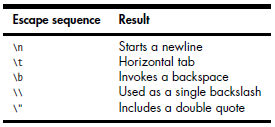
\includegraphics[width=6cm]{Screenshot_3}
%\end{figure}
%
%
%\end{frame}
%
%
%
%\begin{frame}[fragile] %%%%%%%%%%%%%%%%%%%%%%% FRAME %%%%%%%%%%%%%%%%%%%%%%%%%%%%
%
%\begin{flushleft}Examples:\end{flushleft}
%
%\begin{verbatim}
%> cat("here is a string\nsplit\tto neww\b\n\n\tlines")
%here is a string
%split	  to neww
%
%	        lines
%
%> cat("I really want a backslash: \\\nand a double 
%quote: \"")
%I really want a backslash: \
%and a double quote: "
%\end{verbatim}
%
%
%\end{frame}
%
%
%
%\begin{frame}[fragile] %%%%%%%%%%%%%%%%%%%%%%% FRAME %%%%%%%%%%%%%%%%%%%%%%%%%%%%
%
%\begin{flushleft} The function \textit{substr} takes a string x and extracts the part of the string between two character positions (inclusive),\end{flushleft}
%
%\begin{verbatim}
%> foo <- "This is a character string!"
%> substr(x=foo,start=21,stop=27)
%[1] "string!"
%
%> substr(x=foo,start=1,stop=4) <- "Here" #replace a word
%> foo
%[1] "Here is a character string!"
%\end{verbatim}
%
%
%\end{frame}
%
%
%
%\begin{frame}[fragile] %%%%%%%%%%%%%%%%%%%%%%% FRAME %%%%%%%%%%%%%%%%%%%%%%%%%%%%
%
%\begin{flushleft} The \textit{sub} function replace the first instance of a substring, while \textit{gsub} function replaces every instance of pattern.\end{flushleft}
%
%\begin{verbatim}
%> bar <- "How much wood could a woodchuck chuck"
%> sub(pattern="chuck",replacement="hurl",x=bar)
%[1] "How much wood could a woodhurl chuck"
%> gsub(pattern="chuck",replacement="hurl",x=bar)
%[1] "How much wood could a woodhurl hurl"
%\end{verbatim}
%
%
%\end{frame}

%\begin{frame}[fragile] %%%%%%%%%%%%%%%%%%%%%%% FRAME %%%%%%%%%%%%%%%%%%%%%%%%%%%%
%
%\begin{flushleft} Let's create the dataset: \end{flushleft}
%
%\begin{verbatim}
%> firstname <- c("Liz","Jolene","Susan","Boris",
%"Rochelle","Tim","Simon","Amy")
%
%> sex.num <- c(0,0,0,1,0,1,1,0)
%
%> sex.char <- c("female","female","female","male","female",
%"male","male","female")
%
%
%> mob <- c("Apr","Jan","Dec","Sep","Nov","Jul","Jul",
%"Jun")
%[1] "Apr" "Jan" "Dec" "Sep" "Nov" "Jul" "Jul" "Jun"
%\end{verbatim}
%
%
%\end{frame}



%\begin{frame}[fragile] %%%%%%%%%%%%%%%%%%%%%%% FRAME %%%%%%%%%%%%%%%%%%%%%%%%%%%%
%
%\begin{flushleft} Encode a vector as a \textit{factor} (convert \textit{integers} or \textit{characters} to \textit{factors}. \textit{Factors} can be used in statistical modeling.)\end{flushleft}
%
%\begin{verbatim}
%> sex.num.fac <- factor(x=sex.num)
%> sex.num.fac
%[1] 0 0 0 1 0 1 1 0
%Levels: 0 1
%> sex.char.fac <- factor(x=sex.char)
%> sex.char.fac
%[1] female female female male female male male female
%Levels: female male
%
%\end{verbatim}
%
%
%\end{frame}




\end{document}




